\section{Kết quả kiểm chứng và thảo luận}\label{sec:results}
\subsection{Phương pháp kiểm chứng}
Kết quả được kiểm chứng ở ba lớp: (1) tính lại các chỉ số trực tiếp từ CSV độc lập với kho, tiền được đổi sang cent nguyên trước khi cộng để tránh sai số nhị phân; (2) chạy đầy đủ pipeline nạp trên PostgreSQL 16 cùng bộ nghiệm thu F1--F7 và các script đối soát; (3) kiểm thử mã (unit test và gọi API). Các số trong chương này đã được tính lại trên kho vừa nạp và khớp với kết quả tính từ CSV. Ngoài thời gian chạy pipeline, báo cáo không đo độ trễ API hay hiệu năng truy vấn.

\begin{table}[H]\centering\small\renewcommand{\arraystretch}{1.15}
\begin{tabularx}{\linewidth}{>{\raggedright\arraybackslash}p{0.5\linewidth}Y}
\toprule Hạng mục & Kết quả\\\midrule
Pipeline nạp đầy đủ (PostgreSQL 16) và nghiệm thu F1--F7 & Hoàn tất trong khoảng 48 giây, đạt.\\
Giả lập lỗi ở bước nghiệm thu & Pipeline dừng, toàn bộ lần nạp bị rollback, kho cũ nguyên vẹn.\\
Đối soát view DSS với \code{fact_sales} delivered & Khớp ở 13.221.498,11 R\$ và 110.197 món.\\
Đối soát OLAP Khu vực/Người bán (nền, roll-up, drill-down, cộng bang, cộng thành phố, dice, top 3 theo bang) & 4/4 đạt.\\
Gọi API bằng Flask test client (Tổng quan, Thời gian, Khu vực/Người bán, Khách hàng, Quyết định) & 31/31 URL hợp lệ trả mã 200; 3 URL tham số sai trả mã 400.\\
Unit test (tính toán DSS, tăng trưởng cùng kỳ, ngưỡng tháng thưa và số tháng tối thiểu của MoM, QoQ, YoY) & 19/19 đạt.\\
\bottomrule\end{tabularx}
\caption{Kết quả kiểm thử}
\end{table}

\subsection{KPI của kho}
\begingroup\small\renewcommand{\arraystretch}{1.15}
\begin{longtable}{p{0.70\linewidth}r}
\caption{KPI của kho}\label{tab:kpi}\\
\toprule Chỉ số & Giá trị\\\midrule\endfirsthead
\toprule Chỉ số & Giá trị\\\midrule\endhead
\bottomrule\endfoot
Đơn hàng (mọi trạng thái) & 99.441 \\
Dòng sản phẩm (mọi trạng thái) & 112.650 \\
Đơn delivered & 96.478 \\
Dòng sản phẩm delivered & 110.197 \\
Khách có đơn delivered & 93.358 \\
Đơn delivered có thanh toán & 96.477 \\
Đơn delivered thiếu thanh toán & 1 \\
Doanh thu hàng delivered (R\$) & 13.221.498,11 \\
Cước delivered (R\$) & 2.198.275,64 \\
Thanh toán delivered (R\$) & 15.422.461,77 \\
AOV trên đơn có thanh toán (R\$) & 159,86 \\
Khách mua một lần & 90.557 \\
Khách mua lại & 2.801 \\
Tỷ lệ khách mua lại (\%) & 3,00 \\
\end{longtable}\endgroup

Doanh thu hàng cộng cước là 15.419.773,75 R\$, thấp hơn tổng thanh toán 2.688,02 R\$. Hai nhóm thước đo ở grain khác nhau và dữ liệu không có quy tắc đối soát kế toán, nên báo cáo không suy đoán nguyên nhân chênh lệch. Một đơn delivered không có dòng payment được giữ NULL, vì vậy AOV chia cho 96.477 đơn có dữ liệu. Tỷ lệ mua lại 3\% chỉ mô tả cửa sổ quan sát trong dataset, không có nghĩa 97\% khách còn lại đã rời bỏ.

\subsection{Thời gian và danh mục}
\begin{table}[H]\centering\small
\begin{tabularx}{\linewidth}{rYrr}
\toprule Năm mua & Phạm vi dữ liệu delivered & Đơn delivered & Doanh thu hàng (R\$)\\\midrule
2016 & Từ 15/09, thiếu tháng 11 & 267 & 40.470,98\\
2017 & Đủ 12 tháng & 43.428 & 5.962.902,01\\
2018 & Đến 29/08 (tháng 1--8) & 52.783 & 7.218.125,12\\
\bottomrule\end{tabularx}
\caption{Tổng hợp theo năm mua}
\end{table}
Ba năm không cùng số tháng nên tăng trưởng được so theo cùng kỳ. Cụ thể, 2018 (tháng 1--8) so với tháng 1--8 của 2017 tăng +141,13\% (2.993.456 $\rightarrow$ 7.218.125 R\$); quý 3/2018 (chỉ có tháng 7--8) so với tháng 4--5 của quý 2 giảm 12,53\%. YoY của 2017 so với 2016 để trống vì chỉ có một cặp tháng hợp lệ (quy tắc ở chương~\ref{sec:olap}), thay vì +4.796\% khi ghép cả các tháng gần như trống; 2016 chỉ là giai đoạn khởi động với vài đơn mỗi tháng nên không mang ý nghĩa kinh doanh. Chuỗi DSS cũng bắt đầu từ 2017 vì khoảng hở 11--12/2016 (mục~\ref{sec:dss-data}).

\begin{figure}[H]\centering
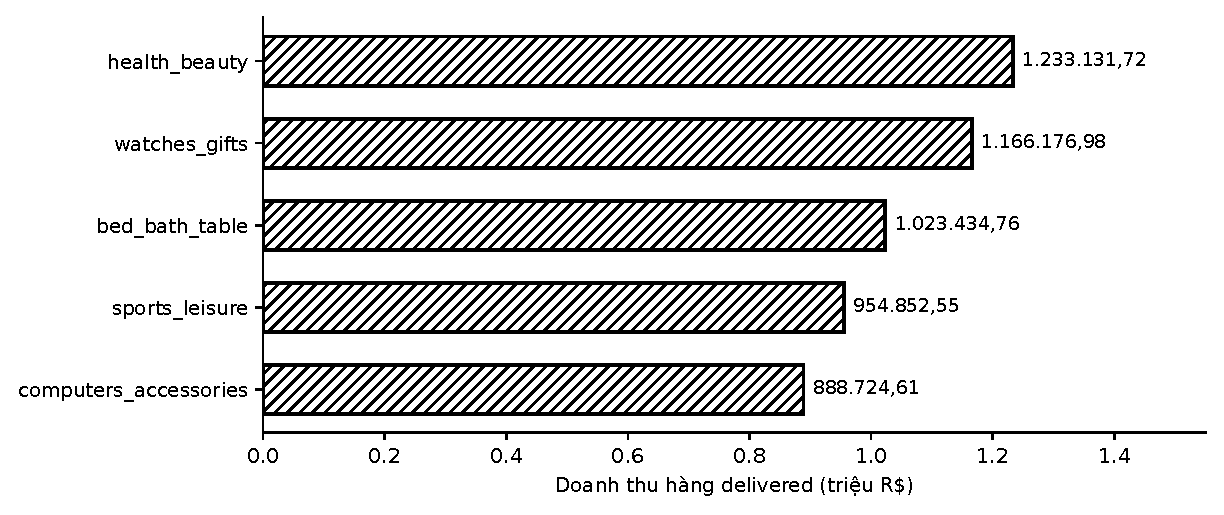
\includegraphics[width=\linewidth]{assets/fig_top_categories.pdf}
\caption{Top 5 danh mục theo doanh thu}
\label{fig:categories}
\end{figure}
Danh mục \code{health_beauty} đứng đầu với 1.233.131,72 R\$, tiếp theo là \code{watches_gifts} và \code{bed_bath_table}. Doanh thu hàng không phải lợi nhuận, nên đây là cơ sở chọn danh mục để phân tích sâu chứ chưa phải căn cứ về hiệu quả kinh doanh.

\subsection{Chất lượng nguồn}
\begin{table}[H]\centering\small
\begin{tabularx}{\linewidth}{YrY}
\toprule Kiểm tra / quan sát & Kết quả & Cách hiểu\\\midrule
Trùng khóa hoặc khóa rỗng ở 7 nguồn nạp & 0 & Theo khóa mà staging khai báo.\\
Orphan ở 5 liên kết nguồn & 0 & Orders--customers; items--orders/products/sellers; payments--orders.\\
Giá, cước, payment âm & 0 & Quan sát từ CSV.\\
Sản phẩm thiếu danh mục & 610 & NULLIF giữ thiếu, không tự gán.\\
Sản phẩm có danh mục chưa có bản dịch & 13 & Hai danh mục \code{pc_gamer} và \code{portateis_cozinha_e_preparadores_de_alimentos}; LEFT JOIN giữ sản phẩm.\\
Đơn thiếu ngày duyệt & 160 & \code{approved_date_key} cho phép NULL.\\
Đơn không có dòng hàng (mọi trạng thái) & 775 & Cardinality order--item là 0..N.\\
\bottomrule\end{tabularx}
\caption{Chất lượng dữ liệu nguồn}
\end{table}

\subsection{Giới hạn của kết luận}
Giao diện được kiểm tra ở mức biên dịch và lớp API; chưa có kiểm thử tự động trên trình duyệt, màn hình hẹp hay nhiều trình duyệt. Chưa có đo hiệu năng. Kết quả DSS dựa trên 14 tháng backtest, và ở mức bang, danh mục mỗi chuỗi chỉ có vài trăm món mỗi tháng, nên chỉ có giá trị ước lượng thô (chương~\ref{sec:dss}).
